\documentclass[10.5pt]{ctexart}
\usepackage{graphicx}
\usepackage{indentfirst}
\usepackage[a4paper, inner=1.5cm, outer=3cm, top=2cm, bottom=3cm, bindingoffset=1cm]{geometry}
\usepackage{epstopdf}
\usepackage{array}
\usepackage{fontspec}
\usepackage{gensymb}
\usepackage[lofdepth,lotdepth]{subfig}
\setlength{\extrarowheight}{4pt}
\begin{document}
\title{\textbf{\fontsize{15.75pt}{\baselineskip}{蒸气压实验报告}}} % 15.75pt is 3 号 in chinese
\author{\fontsize{12pt}{\baselineskip}{数33 赵丰 2013012178 \quad 助教:韩强}}
\date{\fontsize{12pt}{\baselineskip}{10 10,2016}}
\maketitle
\section{\textbf{\fontsize{12pt}{\baselineskip}{引言}}}
本次实验用静态法测定乙醇的饱和蒸气压。根据\textbf{Claperyron} 方程纯液体饱和蒸气压与温度的关系为:
\begin{equation}
\frac{d \ln p}{dT}=\frac{\Delta H_m}{RT_2}
\end{equation}
当温度变化范围不大时,液体的摩尔汽化热$\Delta H_m$可近似认为不变,此时上式可化为:
\begin{equation}
\ln p=-\frac{\Delta H_m}{RT}+A
\end{equation}
通过测定不同温度下乙醇的饱和蒸气压,作图$\ln p-\frac{1}{T}$,线性回归可得液体的摩尔汽化热。
\section{\textbf{\fontsize{12pt}{\baselineskip}{实验操作}}}
\subsection{\textbf{\fontsize{12pt}{\baselineskip}{实验药品、仪器型号及测试装置简图}}}
本次实验用到的主要仪器如下图所示:
\begin{figure}[!ht]
\centering
\caption{蒸气压实验主要装置模式图}
\includegraphics[width=350pt]{VaporTemperatureTest.pdf}
\end{figure}


图中等位计烧瓶部分为乙醇作为被测样品,其沸腾时的饱和蒸气压与B部分乙醇蒸气的压力相等,U型管部分盛有乙醇作为封闭液。
实验装置中各部分的作用:\newline
冷凝管:保证从等位计蒸发的乙醇蒸气冷凝回流到等位计中。\newline
干燥管:防止安全瓶中的水分挥发进入等位计使乙醇样品不纯。
\subsection{\textbf{\fontsize{12pt}{\baselineskip}{实验条件}}}
本次实验的实验装置压力变化范围为25kPa到70kPa,温度变化范围是45 \degree C到70 \degree C。
\subsection{\textbf{\fontsize{12pt}{\baselineskip}{实验操作步骤及方法要点}}}
\begin{enumerate}
\item 连接好装置后,接通真空泵抽气,通过观察气压计示数是否明显降低判断装置是否漏气,待气压计的示数降到25kPa左右时停止抽气,打开稳压瓶和负压瓶之间的活塞,以保留负压瓶中的气体以便备用。
\item 赶走等位计B部分的空气,方法是水浴加热等位计到烧瓶中的乙醇沸腾,可将空气带出。
\item 随着水浴温度的升高,每到等位计的乙醇液体沸腾时可打开放气活塞向稳压瓶中放入空气,将封闭液下压,从而减小了B部分乙醇蒸气的体积,使乙醇蒸气的压强增大,大于该温度下乙醇的饱和蒸气压,从而使沸腾现象停止,每隔2到3 \degree C,记录一次温度和压力的数值,由于实验条件的限制,压力的读数并不是乙醇样品的饱和蒸气压,但由于封闭液两侧高度差对压强的贡献相比于稳压瓶的压强小得多,可以近似把气压计的读数当成乙醇样品的饱和蒸气压。
\end{enumerate}
\section{\textbf{\fontsize{12pt}{\baselineskip}{结果与讨论}}}
\subsection{\textbf{\fontsize{12pt}{\baselineskip}{原始实验数据}}}
按照引言中所述,根据实验数据$\ln p-\frac{1}{T}$作图得到:
\begin{figure}[!ht]
  \centering
  \caption{乙醇的饱和蒸气压随温度变化关系}
  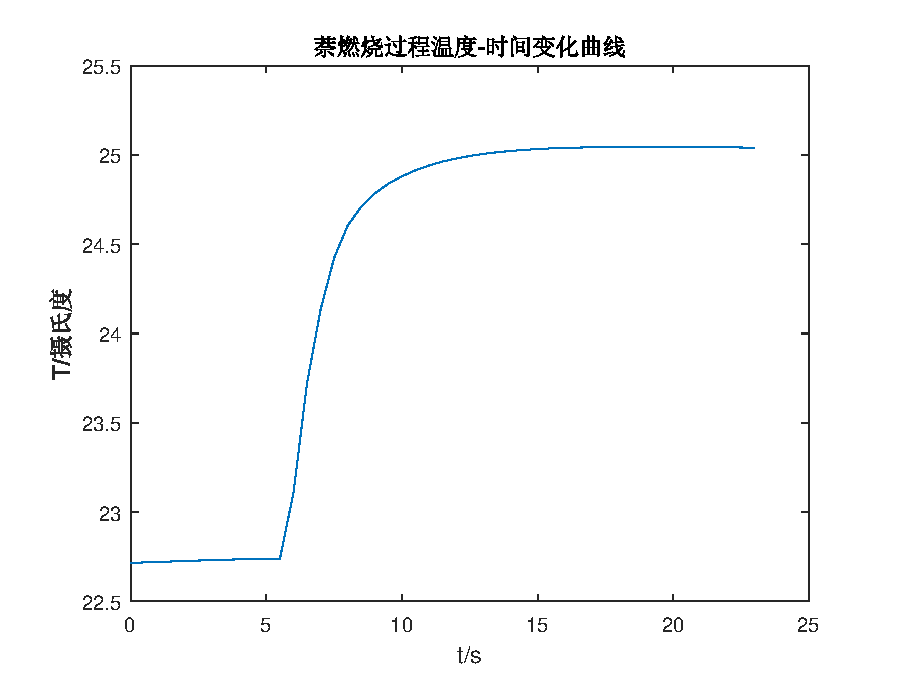
\includegraphics[height=6cm]{figure2.eps}
\end{figure}

\subsection{\textbf{\fontsize{12pt}{\baselineskip}{计算的数据、结果}}}

线性回归直线的斜率为$\frac{\Delta H_m}{R}$,由此计算出的
$\Delta H_m =43.4kJ/mol$,文献值为38.6kJ/mol
将p=103.15kPa代入直线方程,可算出乙醇的正常沸点为77.2\degree C.
文献值为78.37 \degree C.
\section{\textbf{\fontsize{12pt}{\baselineskip}{实验的改进
}}}
实验参考步骤给出的通过放气调节内外压差相等的方法不足为信,因为调整后等位计B部分的压力不是饱和蒸气压。为此,可考虑在液体沸腾时(这时由于B部分压力等于饱和蒸气压不变,U形管液柱高度差不变,可通过测量高度差算出B部分和稳压瓶中的气压差,从而间接地求出液体的饱和蒸气压。
另外,本实验还可以通过改变稳压瓶中的气压,先固定压力,再把待测液体加热到沸腾,记录温度的方法,这时可近似认为固定的压力(即气压计的示数)为饱和蒸气压。如果需要进一步精确,则只需再考虑U形管液柱高度差的影响。这种方法也被称为动态法。
\section{\textbf{\fontsize{12pt}{\baselineskip}{参考文献}}}
\begin{thebibliography}{}
\bibitem{Bib1}物理化学实验 \quad 化学工业出版社
\end{thebibliography}
\end{document}